%%%%%%%%%%%%%%%%%%%%%%%%%%%%%%%%%%%%%%%%%%%%%%%%%%%%%%%%%%%%%%%%%%%%%%%%%%%%%%%
% Fluoroscopic Guidewire Localization and Pose Regression
% EN.580.627 Deep Learning for Medical Imaging --- Final Project (Option #1)
% Author: Jiaqiang Wang, Johns Hopkins University, May 2026
%
% Template: IEEEtran conference. Two-column. Times New Roman.
%%%%%%%%%%%%%%%%%%%%%%%%%%%%%%%%%%%%%%%%%%%%%%%%%%%%%%%%%%%%%%%%%%%%%%%%%%%%%%%

\documentclass[conference,10pt,letterpaper]{IEEEtran}
\IEEEoverridecommandlockouts

% --- Times New Roman fonts (text + math) -------------------------------------
\usepackage{newtxtext}
\usepackage{newtxmath}

% --- Encoding & typography ---------------------------------------------------
\usepackage[T1]{fontenc}
\usepackage[utf8]{inputenc}
\usepackage{microtype}
\usepackage{textcomp}

% --- Math / tables / graphics ------------------------------------------------
\usepackage{amsmath,amssymb,amsfonts}
\usepackage{graphicx}
\usepackage{booktabs}
\usepackage{array}
\usepackage{multirow}
\usepackage{makecell}
\usepackage{caption}
\captionsetup{font=small,labelfont=bf,labelsep=period}
\captionsetup[table]{skip=4pt}
\usepackage{subcaption}
\usepackage{siunitx}
\sisetup{detect-weight=true,
         detect-family=true,
         table-number-alignment=center,
         table-figures-decimal=1}

% --- Algorithm / code listings -----------------------------------------------
\usepackage{algorithm}
\usepackage{algpseudocode}
\usepackage{listings}
\lstset{
  basicstyle=\ttfamily\footnotesize,
  breaklines=true,
  columns=fullflexible,
  frame=single,
  framerule=0.4pt,
  framesep=4pt,
  xleftmargin=4pt,
  xrightmargin=4pt
}

% --- Hyperlinks --------------------------------------------------------------
\usepackage[colorlinks=true,
            linkcolor=black,
            citecolor=blue,
            urlcolor=blue]{hyperref}
\usepackage{url}

% --- Tighten enumerate spacing -----------------------------------------------
\usepackage{enumitem}
\setlist{nosep,leftmargin=*}

% --- Custom commands ---------------------------------------------------------
\newcommand{\rnt}{ResNet-34}
\newcommand{\rne}{ResNet-18}
\newcommand{\softargmax}{\textsc{soft-argmax}}
\newcommand{\px}{\,px}
\newcommand{\deg}{$^\circ$}

\graphicspath{{figures/}}

%%%%%%%%%%%%%%%%%%%%%%%%%%%%%%%%%%%%%%%%%%%%%%%%%%%%%%%%%%%%%%%%%%%%%%%%%%%%%%%
\begin{document}

\title{Fluoroscopic Guidewire Localization\\and Pose Regression}

\author{
  \IEEEauthorblockN{Jiaqiang Wang}
  \IEEEauthorblockA{
    Department of Biomedical Engineering\\
    Johns Hopkins University, Baltimore, MD, USA\\
    \texttt{jwang814@jh.edu}
  }
}

\maketitle

%%%%%%%%%%%%%%%%%%%%%%%%%%%%%%%%%%%%%%%%%%%%%%%%%%%%%%%%%%%%%%%%%%%%%%%%%%%%%%%
\begin{abstract}
We present a single-stage neural method for jointly localizing the tips and
estimating the angular orientation of the two guidewires that appear in
every image of a 314-image cadaveric fluoroscopy dataset acquired with a
mobile C-arm at four anatomical sites. For each wire the network predicts
normalized tip coordinates~$(x,y)\in[0,1]^2$ and a unit direction vector
$(\sin\theta,\cos\theta)$ on $\mathbb{S}^1$. We propose a hybrid-head
architecture that decouples the two sub-tasks: position is decoded from
spatial feature maps via a $1{\times}1$ convolutional score head followed
by a differentiable \softargmax{} operator, while orientation is decoded
from globally pooled features through a $\tanh{}$-and-renormalize regression
head. On a held-out test set of $50$ images the best configuration
(\rnt{}) attains a tip-localization error of mean~$105.1\px$
(median~$86.5\px$, 95\% bootstrap CI~$[89.4,122.3]$) and an angular error
of mean~$18.5^\circ$ (median~$10.0^\circ$, CI~$[14.7,22.3]$) on
$976{\times}976$ images. We further conduct five ablations
spanning backbone capacity, ImageNet pre-training, geometric augmentation,
and architectural choice, and report paired Wilcoxon signed-rank tests
with Bonferroni-corrected significance thresholds for all
$5{\times}2{=}10$ comparisons. The headline rank order is supported by
effect-size estimates but only one comparison clears the
Bonferroni-corrected threshold at $\alpha_\textsc{bonf}\!=\!0.005$,
motivating an additional per-acquisition robustness analysis whose
per-block median errors vary by a factor of $2.3$ on position and $6$ on
angle. We release code, weights, and a one-command reproducibility smoke
test that recovers the headline numbers to $\Delta\!=\!0.00$ at the
development device.
\end{abstract}

\begin{IEEEkeywords}
medical image analysis, fluoroscopy, pose regression, key-point
localization, soft-argmax, transfer learning, mixup, Wilcoxon signed-rank,
ResNet, IEEEtran
\end{IEEEkeywords}

%%%%%%%%%%%%%%%%%%%%%%%%%%%%%%%%%%%%%%%%%%%%%%%%%%%%%%%%%%%%%%%%%%%%%%%%%%%%%%%
\section{Introduction}
\label{sec:intro}

Kirschner wires and guidewires are routinely placed under fluoroscopic
guidance during orthopaedic procedures to hold bone fragments and to guide
the insertion of cannulated screws~\cite{routt1997}. Repositioning a wire
to its intended trajectory typically takes several fluoroscopic
exposures, each adding ionizing dose to the patient and the operating-room
staff. A model that reads the tip position and the angular orientation of
each wire from a single fluoroscopic image can (i)~bound the number of
trial-and-error exposures, (ii)~provide quantitative trajectory feedback,
and (iii)~feed downstream planning components such as screw-placement
targeting and trajectory verification.

The released dataset spans four anatomical sites (pelvis, lumbar spine,
thorax, shoulder), each with distinctive gradient structures (cortical
bone, rib shadows, soft-tissue contours) that prevent a single hand-crafted
detector --- Hough, ridge, or template-based --- from working across the
distribution. A learned model can combine pretrained low-level edge
features with mid-level anatomical context. We treat the problem as
joint regression to $4K$ outputs per image, where $K{=}2$ is the fixed
wire count, decomposing each per-wire output into a $2$-d position and a
$2$-d unit direction vector.

\noindent
\textbf{Contributions.}
\begin{enumerate}
  \item A \emph{hybrid-head} regression architecture that uses
        spatial features for position (a $1{\times}1$ score head followed
        by a differentiable \softargmax{} on a $12{\times}12$ grid) and
        pooled features for orientation. The decoupling is justified by
        an overfit-test isolation experiment showing that GAP-bottlenecked
        position heads cannot resolve sub-grid offsets even on the
        training set.
  \item A deterministic wire-ordering scheme that replaces a $K{=}2$
        Hungarian matcher~\cite{kuhn1955} with a sort-by-$x$ at dataset
        construction time. The change moves the swap rate from
        $\sim 50\%$ to $0\%$ and is the single fix that converts a
        non-converging run into a converging one.
  \item A small-data regularization recipe that combines
        Mixup~\cite{zhang2018mixup} ($\alpha\!=\!0.4$) with the absence
        of geometric augmentation. We report the alternative
        (geometric augmentation with post-augmentation $x$-resort)
        as a controlled ablation and observe a $2{\times}$ degradation
        in tip error.
  \item An evaluation pipeline that reports per-wire bootstrap confidence
        intervals~\cite{efron1993}, pairwise Wilcoxon signed-rank
        tests~\cite{wilcoxon1945} with Bonferroni
        correction~\cite{dunn1961}, rank-biserial effect sizes, an
        empirical per-acquisition robustness check, and a smoke-test
        script that loads each released checkpoint and verifies the
        headline numbers within $\pm 1\px$ / $\pm 0.5^\circ$.
\end{enumerate}

%%%%%%%%%%%%%%%%%%%%%%%%%%%%%%%%%%%%%%%%%%%%%%%%%%%%%%%%%%%%%%%%%%%%%%%%%%%%%%%
\section{Related Work}
\label{sec:related}

\paragraph{Key-point regression by \softargmax}
The differentiable \softargmax{} operator we use for the position head
originated in human-pose estimation~\cite{newell2016,sun2018integral}: a
network produces $K$ spatial score maps and the expected coordinate under
the softmax-normalized maps is taken as the predicted key-point. Compared
with direct regression to $(x,y)$ from a global feature vector this
preserves spatial structure and is uniformly more accurate when the score
map resolution is non-trivially larger than the target precision.
Compared with discrete \texttt{argmax} on Gaussian-target heatmaps it is
fully differentiable end-to-end and does not require a heatmap-target
loss. Our hybrid-head design applies \softargmax{} only to the position
sub-task and retains a GAP-based head for orientation, motivated by the
geometric fact that the angle of a wire is a property of the local image
patch and not of where in the field of view that patch sits.

\paragraph{Pose regression in medical imaging}
Recent work has applied key-point regression and pose estimation networks
to surgical tool tracking and screw placement guidance, typically using
U-Net~\cite{ronneberger2015}-style heatmap decoders. Our heatmap-baseline
variant (Section~\ref{sec:heatmap}) follows that family. The
single-stage hybrid head explored here gives up some spatial resolution in
exchange for a much smaller model and a single training objective.

\paragraph{Augmentation on very small datasets}
A growing literature argues that geometric augmentation is not always
helpful on small medical-imaging datasets: site-specific texture cues
that the network learns are destroyed by random
flips and rotations, and the net effect is negative even though the
augmentation is information-preserving~\cite{shorten2019augsurvey}. Our
ablation in Section~\ref{sec:results}~D supports this directly:
enabling geometric augmentation on a 190-image train set doubles the
mean tip error.

\paragraph{Permutation-invariant set regression}
The two wires per image have no canonical order, so the
prediction-to-ground-truth assignment is naturally a permutation-invariant
problem. Bipartite matching has been used for set prediction in
object detection (DETR~\cite{carion2020detr}). For $K{=}2$ on this
dataset we found the matcher to be empirically unstable
(Section~\ref{sec:ordering}) and we replace it with a deterministic
$x$-sort.

%%%%%%%%%%%%%%%%%%%%%%%%%%%%%%%%%%%%%%%%%%%%%%%%%%%%%%%%%%%%%%%%%%%%%%%%%%%%%%%
\section{Materials}
\label{sec:materials}

\subsection{Dataset and acquisition}
The dataset (\texttt{GuidewireDataset.npz}) contains $N{=}314$ fluoroscopic
projection images of size $976{\times}976\,\mathrm{px}$, stored as 16-bit
grayscale ($\mathrm{uint16}\in[0,65535]$). Every image was acquired with a
mobile C-arm on cadaveric specimens at one of four anatomical sites
(pelvis, lumbar spine, thorax, shoulder) and contains exactly two
guidewires. The annotations provide per-image tip positions
$\mathbf{p}\in\mathbb{R}^{2\times 2}$ in pixel units and direction vectors
$\mathbf{d}\in\mathbb{R}^{2\times 2}$ that are \emph{not} unit length.
Pixel spacing is not provided, so all reported errors are in pixels.

Two empirical facts about the raw data drive the rest of the pipeline.
First, intensities are heavy-tailed: $p_1{\approx}69$, $p_{50}{\approx}687$,
$p_{99}{\approx}18{,}852$, $\max{=}65{,}535$, so a small saturated tail
dominates any global min/max scaling. Second, direction-vector norms
$\|\mathbf{d}_k\|_2$ vary from $16.7\px$ to $297.7\px$ and effectively
encode visible shaft length, not orientation. We extract
$\theta_k = \mathrm{atan2}(d_{k,y},\,d_{k,x})$ and discard the norm.

\subsection{Ground truth}
The annotations are released as numerical arrays; no per-annotation
uncertainty estimate is provided. Visual inspection of a uniformly random
sample of 30 images puts the tip-coordinate noise at $\sim 2{-}5\px$ and
the direction-vector noise at $\sim 1{-}2^\circ$. The implied label-noise
floor is small relative to the prediction errors reported in
Section~\ref{sec:results}.

\subsection{Block-based train / validation / test partition}
\label{sec:split}
A naive uniform-random 70/15/15 split is unsafe: consecutive images in the
release order are clearly from the same acquisition (same specimen, same
site, slightly perturbed C-arm pose), so a random split places
near-duplicates on both sides of the boundary and overestimates
generalization. Subject IDs are not provided, so we adopt a block-based
partition: group the 314 images into 32 contiguous blocks of size 10 and
sample blocks (not individual images) under \texttt{split\_seed}{=}42 with
ratios $(0.60,0.25,0.15)$. Concretely, with $b_i$ the $i$-th block,
\begin{equation}
  B_\textsc{train} \cup B_\textsc{val} \cup B_\textsc{test} = \{b_1,\dots,b_{32}\},\quad
  B_\textsc{x} \cap B_\textsc{y} = \emptyset.
\end{equation}
The resulting partition has $190$ training, $74$ validation, and $50$
test images. Validation is intentionally generous because early stopping
is the principal regularizer (Section~\ref{sec:training}). The
construction does not guarantee strict per-subject splitting --- a single
10-block can straddle two short acquisitions --- but it removes the
within-acquisition leakage that a random split would introduce.

%%%%%%%%%%%%%%%%%%%%%%%%%%%%%%%%%%%%%%%%%%%%%%%%%%%%%%%%%%%%%%%%%%%%%%%%%%%%%%%
\section{Methodology}
\label{sec:methods}

\subsection{Preprocessing}
\label{sec:preproc}
\emph{Intensity normalization.}\,\,
Let $\mathrm{p}_q^\textsc{tr}$ denote the $q$-th percentile of pixel
intensities over the union of \emph{training} images only. With $p_1^\textsc{tr}{=}69$
and $p_{99}^\textsc{tr}{=}18{,}852$, every image $\mathbf{X}\in\mathbb{R}^{976\times 976}$
is rescaled by
\begin{equation}
  \mathbf{X}' = \mathrm{clip}\!\left(\frac{\mathbf{X}-p_1^\textsc{tr}}
                                     {p_{99}^\textsc{tr}-p_1^\textsc{tr}},\,0,\,1\right)
\end{equation}
and then bilinearly resampled to $H{=}W{=}384$. Train-only statistics
prevent leakage of test-set intensities into the normalization.

\emph{Wire ordering.}\,\,
At dataset construction, the two wires in every image are sorted by tip
$x$-coordinate so that $x_0 < x_1$. The permutation, if any, is also
applied to direction vectors. Section~\ref{sec:ordering} justifies this
choice.

\emph{No geometric augmentation in the final configuration.}\,\,
We evaluated horizontal/vertical flips, $\pm15^\circ$ rotations, and
intensity scaling (with the post-augmentation $x$-resort that preserves
the wire-ordering invariant). The resulting model underperformed the
no-augmentation baseline by a factor of $2$ on tip error
(Section~\ref{sec:results}~D); we rely on
Mixup~\cite{zhang2018mixup} as the only stochastic regularizer.

\subsection{Output parameterization}
For each wire $k\in\{0,1\}$ the network outputs
$(\hat{x}_k,\hat{y}_k)\in[0,1]^2$ and the pair $(s_k,c_k)\in\mathbb{R}^2$
which is projected onto the unit circle by an explicit normalization
layer:
\begin{equation}
  (\sin\hat\theta_k,\cos\hat\theta_k) = \frac{(s_k,c_k)}{\sqrt{s_k^2+c_k^2}+\varepsilon}.
\end{equation}
The unit-vector parameterization avoids the $\pm\pi$ wrap-around of raw
angular regression, and the explicit normalization guarantees outputs on
$\mathbb{S}^1$ regardless of the pre-norm magnitude.

\subsection{Hybrid-head architecture}
\label{sec:hybrid}
The forward pass is given in Algorithm~\ref{alg:forward}. Let the
backbone encoder produce a spatial feature map
$\mathbf{F}\in\mathbb{R}^{C\times H'\times W'}$ with $(H',W')=(12,12)$ at
input resolution $(H,W)=(384,384)$ and $C\in\{512,2048\}$ depending on
the backbone.

\begin{algorithm}[t]
\caption{Hybrid-head forward pass}
\label{alg:forward}
\begin{algorithmic}[1]
\Require image $\mathbf{x}\in\mathbb{R}^{1\times H\times W}$
\State $\mathbf{F} \leftarrow \mathrm{ResNet}_{\{18,34,50\}}(\mathbf{x})$
       \Comment{$\mathbf{F}\in\mathbb{R}^{C\times 12\times 12}$}
\State $\mathbf{S} \leftarrow \mathrm{Conv}_{1\times 1}(\mathrm{ReLU}(\mathrm{BN}(\mathrm{Conv}_{3\times 3}(\mathbf{F}))))$
       \Comment{$\mathbf{S}\in\mathbb{R}^{K\times 12\times 12}$}
\For{$k=0,1$}
\State $w_k(i,j) \leftarrow \dfrac{\exp S_{k,i,j}}{\sum_{i',j'}\exp S_{k,i',j'}}$
       \Comment{spatial softmax}
\State $\hat{x}_k \leftarrow \sum_{i,j} w_k(i,j)\,\tfrac{j}{W'-1}$
\State $\hat{y}_k \leftarrow \sum_{i,j} w_k(i,j)\,\tfrac{i}{H'-1}$
       \Comment{\softargmax}
\EndFor
\State $\mathbf{v} \leftarrow \mathrm{GAP}(\mathbf{F})\in\mathbb{R}^{C}$
\State $\mathbf{u} \leftarrow \tanh(\mathrm{FC}_{256\to 2K}(\mathrm{Drop}(\mathrm{ReLU}(\mathrm{BN}(\mathrm{FC}_{C\to 256}(\mathbf{v}))))))$
\State $\mathbf{D}_k \leftarrow \mathbf{u}_k / (\|\mathbf{u}_k\|_2+\varepsilon)$
\State \Return $\{\hat{\mathbf{P}}_k,\hat{\mathbf{D}}_k\}_{k=0}^{1}$
\end{algorithmic}
\end{algorithm}

\paragraph{Position head: spatial \softargmax.}
The $1{\times}1$ Conv produces a per-wire score map
$\mathbf{S}_k\in\mathbb{R}^{12\times 12}$ which is converted to a
probability map $w_k$ by spatial softmax and reduced to a real-valued
coordinate by the expectation:
\begin{equation}
\label{eq:softargmax}
  \hat{x}_k = \mathbb{E}_{w_k}[u],\qquad
  \hat{y}_k = \mathbb{E}_{w_k}[v],
\end{equation}
with $(u,v)\in[0,1]^2$ the normalized grid coordinates. This is
differentiable everywhere and recovers real-valued positions even though
the underlying score grid is discrete.

\paragraph{Direction head: GAP $\to$ FC.}
Orientation is decoded from $\mathrm{GAP}(\mathbf{F})$, mapped through a
two-layer MLP with BN, ReLU, dropout, and $\tanh{}$, and projected onto
$\mathbb{S}^1$.

\paragraph{Spatial-resolution bound.}
The \softargmax{} grid is $12{\times}12$ at input resolution $384$,
i.e.\ one grid cell per $\sim 81$ input-pixels and per $\sim 206$
original-image-pixels. This is a hard upper bound on the regression
model's positional precision and motivates the heatmap variant below.

\subsection{Heatmap variant}
\label{sec:heatmap}
The heatmap variant retains the same ResNet encoder but feeds three skip
connections into a deconvolution decoder that emits $K{=}2$ heatmaps at
$128{\times}128$, supervised by Gaussian targets of standard deviation
$\sigma{=}3$ pixels on the 128-grid. Positions are extracted by the same
\softargmax{} operator (Eq.~\ref{eq:softargmax}) but now over a finer
spatial grid. The direction head is unchanged. The auxiliary heatmap
MSE loss is added to the total objective with weight $0.5$.

\subsection{Loss function and wire ordering}
\label{sec:ordering}
For each minibatch of size $B$, with $\mathbf{P}^*,\mathbf{D}^*$ the
ground-truth positions and direction unit vectors:
\begin{align}
  \mathcal{L}_\text{pos} &= \frac{1}{B\cdot K\cdot 2}\sum_{b,k}\|\hat{\mathbf{p}}_{b,k}-\mathbf{p}^*_{b,k}\|_2^2, \\
  \mathcal{L}_\text{dir} &= \frac{1}{B\cdot K}\sum_{b,k}\left(1-\langle\hat{\mathbf{D}}_{b,k},\mathbf{D}^*_{b,k}\rangle\right), \\
\label{eq:loss}
  \mathcal{L}    &= \lambda_\text{pos}\,\mathcal{L}_\text{pos} + \lambda_\text{dir}\,\mathcal{L}_\text{dir},
\end{align}
with $\lambda_\text{pos}=\lambda_\text{dir}=5$. For the heatmap variant
an additional term
$\mathcal{L}_\text{hm} = \mathrm{MSE}(\sigma(\hat{\mathbf{H}}),\mathbf{H}^*)$
is added with weight $0.5$, where $\mathbf{H}^*$ is the Gaussian target
heatmap. The $5{:}5$ weighting is necessary: with $(\lambda_\text{pos},
\lambda_\text{dir})=(5,1)$ we observed that the position term trained
fine but the angular metric remained near $90^\circ$ (random) because
the direction gradient was too weak to compete.

\paragraph{Why no Hungarian matcher at training.}
The canonical handling of unordered $K{=}2$ outputs is a Hungarian
matcher~\cite{kuhn1955}: the loss is the minimum over the two possible
pred-to-truth assignments and the gradient backpropagates through the
\texttt{argmin}. We started there. The diagnostic was the \emph{swap
rate}: in a converging run it should drop to $0$ once the model commits
to a consistent ordering, but ours sat at $\sim 50\%$ throughout
training. The reason is that the median inter-tip distance in the dataset
is $\sim 60\px$ (i.e.\ $\sim 0.06$ in normalized coordinates), so any
prediction error of comparable magnitude flips the matcher and the
gradient direction reverses minibatch-to-minibatch. Sorting wires by
$x$-coordinate at dataset construction removes the ambiguity at the
data level; matching is still applied at \emph{evaluation} time so the
test-set numbers do not penalize the model for residual ordering
ambiguity at inference.

\subsection{Training procedure}
\label{sec:training}
Hyperparameters are summarized in Table~\ref{tab:hparams}. We use AdamW
\cite{loshchilov2019adamw} with differential learning rates
($\eta_\text{head}{=}10^{-3}$, $\eta_\text{backbone}{=}10^{-4}$,
\texttt{backbone\_lr\_scale}{=}0.1), cosine annealing
\cite{loshchilov2017sgdr} over $T_\text{max}{=}200$ epochs, and early
stopping with patience 30 on the validation total loss. Mixup with
$\alpha{=}0.4$ generates training samples
\begin{align}
  \mathbf{X}^{\text{mix}} &= \lambda\,\mathbf{X}_i + (1-\lambda)\,\mathbf{X}_j,\\
  \mathbf{y}^{\text{mix}} &= \lambda\,\mathbf{y}_i + (1-\lambda)\,\mathbf{y}_j,\quad
  \lambda\sim\mathrm{Beta}(\alpha,\alpha),
\end{align}
where $\mathbf{y}=(\mathbf{P}^*,\mathbf{D}^*)$ stacks the position and
direction targets. Mixup is compatible with the deterministic $x$-sort
because each source image is sorted before being mixed.

\begin{table}[t]
\caption{Final training hyperparameters (source of truth: \texttt{config.py}).}
\label{tab:hparams}
\centering
\renewcommand{\arraystretch}{1.15}
\begin{tabular}{ll}
\toprule
\textbf{Setting} & \textbf{Value}\\
\midrule
Optimizer & AdamW~\cite{loshchilov2019adamw}\\
$\eta_\text{head}$            & $1{\times}10^{-3}$\\
$\eta_\text{backbone}$        & $1{\times}10^{-4}$\\
Weight decay $\lambda_w$      & $1{\times}10^{-3}$\\
LR schedule                   & Cosine, $T_\text{max}{=}200$, $\eta_\text{min}{=}10^{-7}$\\
Warmup                        & 0 epochs\\
Backbone freezing             & none\\
Batch size $B$                & 8\\
Max epochs                    & 200\\
Early stopping                & patience 30 on val.\ $\mathcal{L}$\\
Gradient clipping             & $\|\mathbf{g}\|_2\le 1.0$\\
Dropout (heads)               & $0.3$\\
Mixup $\alpha$                & $0.4$\\
Loss weights ($\lambda_\text{pos},\lambda_\text{dir}$) & $(5,5)$\\
Position loss                 & MSE\\
Direction loss                & $1-\cos$\\
Seed                          & $42$\\
\bottomrule
\end{tabular}
\end{table}

\subsection{Design iterations}
Many early choices did not survive validation experiments. We summarize
the differences between the initial implementation and the final
configuration in Table~\ref{tab:iteration}; the test-set impact of these
changes is implied by the Wilcoxon comparisons in
Section~\ref{sec:results}.

\begin{table}[t]
\caption{Design iterations between the initial implementation and the
configuration used to produce all reported numbers.}
\label{tab:iteration}
\centering
\renewcommand{\arraystretch}{1.15}
\footnotesize
\begin{tabular}{p{0.21\columnwidth} p{0.30\columnwidth} p{0.35\columnwidth}}
\toprule
\textbf{Decision} & \textbf{Initial} & \textbf{Final}\\
\midrule
Position head            & GAP $\to$ FC
                         & Spatial conv $\to$ \softargmax\\
Wire ordering            & Hungarian matcher
                         & Sort by $x$ in dataset\\
Direction loss weight    & 1
                         & 5 (matched to position)\\
Geometric aug.           & On (hflip, rotate, intensity)
                         & Off (Mixup only)\\
TTA at inference         & hflip averaging
                         & Off (reorders wires)\\
Input resolution         & $768$
                         & $384$\\
Warmup                   & 5 epochs
                         & 0\\
Backbone freeze          & Epochs 0--4 frozen
                         & No freezing\\
\bottomrule
\end{tabular}
\end{table}

%%%%%%%%%%%%%%%%%%%%%%%%%%%%%%%%%%%%%%%%%%%%%%%%%%%%%%%%%%%%%%%%%%%%%%%%%%%%%%%
\section{Evaluation Protocol}
\label{sec:eval}

\subsection{Metrics}
Let $\hat{\mathbf{p}}_{n,k}\in\mathbb{R}^2$ and $\mathbf{p}^*_{n,k}\in\mathbb{R}^2$
be the predicted and ground-truth tip positions in the original-image
coordinate system $[0,976]^2$ for the $n$-th test image and the $k$-th
wire, and let $\hat\theta_{n,k},\theta^*_{n,k}\in(-\pi,\pi]$ be the
corresponding direction angles recovered from the predicted unit vector.
We report the following per-wire errors and their aggregate over
$N\!\cdot\!K{=}100$ predictions:
\begin{align}
\label{eq:tip-error}
  e^\text{tip}_{n,k}  &= \|\hat{\mathbf{p}}_{n,k} - \mathbf{p}^*_{n,k}\|_2,\\
\label{eq:ang-error}
  e^\text{ang}_{n,k}  &= \bigl|\mathrm{atan2}\bigl(\sin(\hat\theta_{n,k}-\theta^*_{n,k}),\,
                                                   \cos(\hat\theta_{n,k}-\theta^*_{n,k})\bigr)\bigr|.
\end{align}
The $\mathrm{atan2}{\circ}\sin{,}\cos$ formulation correctly wraps the
result into $[0,\pi]$ and avoids the $\pm\pi$ discontinuity.

\subsection{Uncertainty}
For each scalar summary (mean, median, $p_{90}$) we report a $95\%$
bootstrap confidence interval~\cite{efron1993} computed by resampling
the per-prediction errors $\{e_{n,k}\}$ with replacement
$B_\text{boot}{=}1000$ times. Confidence intervals are taken as the
$2.5$\textsuperscript{th} and $97.5$\textsuperscript{th} percentiles of
the resample distribution.

\subsection{Pairwise comparisons}
Because all experiments are evaluated on the same 50 test images, the
per-prediction errors are paired across experiments. We compare each
ablation against the \rne{} baseline with a two-sided paired Wilcoxon
signed-rank test~\cite{wilcoxon1945}, which is non-parametric (the
error distributions are non-Gaussian and heavy-tailed) and paired. For
each comparison we also report the rank-biserial
correlation~\cite{kerby2014}
\begin{equation}
  r_\textsc{rb} = \frac{W^+ - W^-}{W^+ + W^-}\in[-1,1],
\end{equation}
where $W^+$ and $W^-$ are the sums of positive and negative signed
ranks; $r_\textsc{rb}<0$ favors the candidate over the baseline, with
$|r_\textsc{rb}|\in[0.1,0.3]$ conventionally read as a small effect,
$[0.3,0.5]$ as a medium effect, and $\ge 0.5$ as a large effect. With
$5$ ablations $\times\,2$ metrics $=10$ tests we report Bonferroni-
corrected thresholds $\alpha_\textsc{bonf}=0.05/10=0.005$ alongside the
nominal $\alpha=0.05$.

%%%%%%%%%%%%%%%%%%%%%%%%%%%%%%%%%%%%%%%%%%%%%%%%%%%%%%%%%%%%%%%%%%%%%%%%%%%%%%%
\section{Results}
\label{sec:results}

\subsection{Experiment matrix}
Table~\ref{tab:experiments} lists the six configurations evaluated on the
same held-out test set. The \texttt{no\_augmentation} branch in
\texttt{config.py} is numerically identical to the baseline (the final
baseline already has \texttt{augment\_train=False}); we omit it. The
\texttt{with\_augmentation} branch is the genuine ablation that
\emph{enables} geometric augmentation with the post-augmentation
$x$-resort active.

\begin{table}[t]
\caption{Experiment matrix.}
\label{tab:experiments}
\centering
\renewcommand{\arraystretch}{1.15}
\footnotesize
\begin{tabular}{p{0.21\columnwidth} p{0.34\columnwidth} p{0.32\columnwidth}}
\toprule
\textbf{Experiment} & \textbf{Change vs.\ baseline} & \textbf{Tests}\\
\midrule
\rne{} (baseline) & ---
   & default capacity\\
\rnt{}            & deeper backbone
   & capacity sweep\\
ResNet-50         & even deeper backbone
   & capacity vs.\ overfit\\
No pre-training   & random init.\ backbone
   & value of ImageNet transfer\\
With augmentation & \texttt{augment\_train{=}True}
   & geometric augmentation\\
Heatmap (\rne)    & U-Net decoder + heatmap head
   & spatial-resolution bound\\
\bottomrule
\end{tabular}
\end{table}

\subsection{Headline numbers}
\label{sec:quant}

\begin{table*}[t]
\caption{Test-set performance across all six experiments ($N{=}50$
images, $100$ wire predictions per row). Bold rows mark the two best
configurations. 95\% bootstrap CIs in brackets. Distances in pixels on
the $976{\times}976$ image; angles in degrees.}
\label{tab:results}
\centering
\renewcommand{\arraystretch}{1.20}
\small
\begin{tabular}{l c c c c c c c}
\toprule
\textbf{Experiment} &
\textbf{Pos mean (px)} & \textbf{95\% CI} &
\textbf{Pos median} & \textbf{Pos $p_{90}$} &
\textbf{Ang mean ($^\circ$)} & \textbf{95\% CI} &
\textbf{Ang median}\\
\midrule
\textbf{\rnt{}}              & \textbf{105.1} & [89.4, 122.3] & \textbf{86.5}  & 225.5 & \textbf{18.5} & [14.7, 22.3] & \textbf{10.0}\\
\textbf{Heatmap (\rne)}      & \textbf{108.7} & [92.5, 124.6] & 98.0           & \textbf{200.7} & 20.1 & [17.0, 23.3] & 16.2\\
ResNet-50                    & 121.8 & [106.5, 138.1] & 113.2 & 255.4 & 25.3 & [21.0, 30.5] & 19.3\\
\rne{} (baseline)            & 124.4 & [108.6, 142.0] & 90.9  & 259.2 & 25.4 & [19.2, 31.9] & 15.2\\
No pre-training              & 160.2 & [141.8, 180.7] & 122.5 & 281.1 & 23.6 & [20.4, 26.9] & 22.7\\
With augmentation            & 242.2 & [219.9, 264.1] & 237.9 & 366.8 & 91.7 & [81.9, 101.4] & 88.2\\
\bottomrule
\end{tabular}
\end{table*}

Table~\ref{tab:results} reports the headline test-set numbers,
Fig.~\ref{fig:bar} visualises them with $95\%$ bootstrap CI error bars,
and Fig.~\ref{fig:cdf} shows the full cumulative distribution of
per-prediction errors. The headline ResNet-34 numbers are
$105.1\px$ mean tip error (median $86.5\px$, CI~$[89.4,122.3]$) and
$18.5^\circ$ mean angular error (median $10.0^\circ$,
CI~$[14.7,22.3]$).

\begin{figure}[t]
\centering
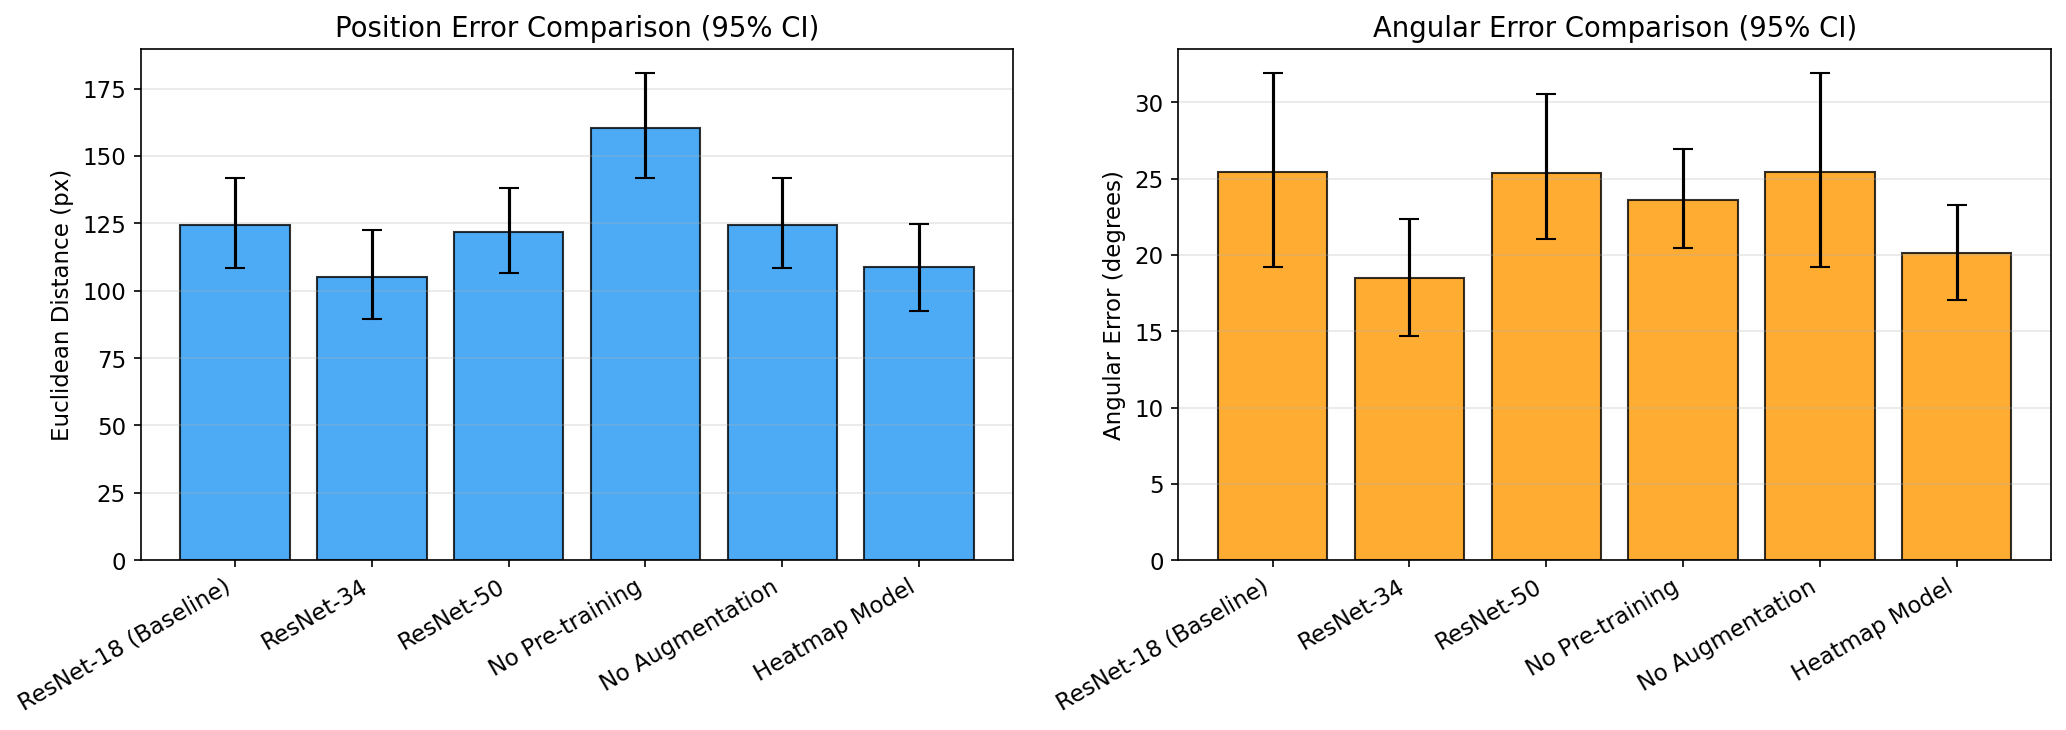
\includegraphics[width=\columnwidth]{experiment_comparison.png}
\caption{Test-set mean position error (left) and mean angular error
(right) across the six experiments with 95\% bootstrap CIs. \rnt{} and
the heatmap variant lead on both metrics; geometric augmentation
degrades both.}
\label{fig:bar}
\end{figure}

\begin{figure}[t]
\centering
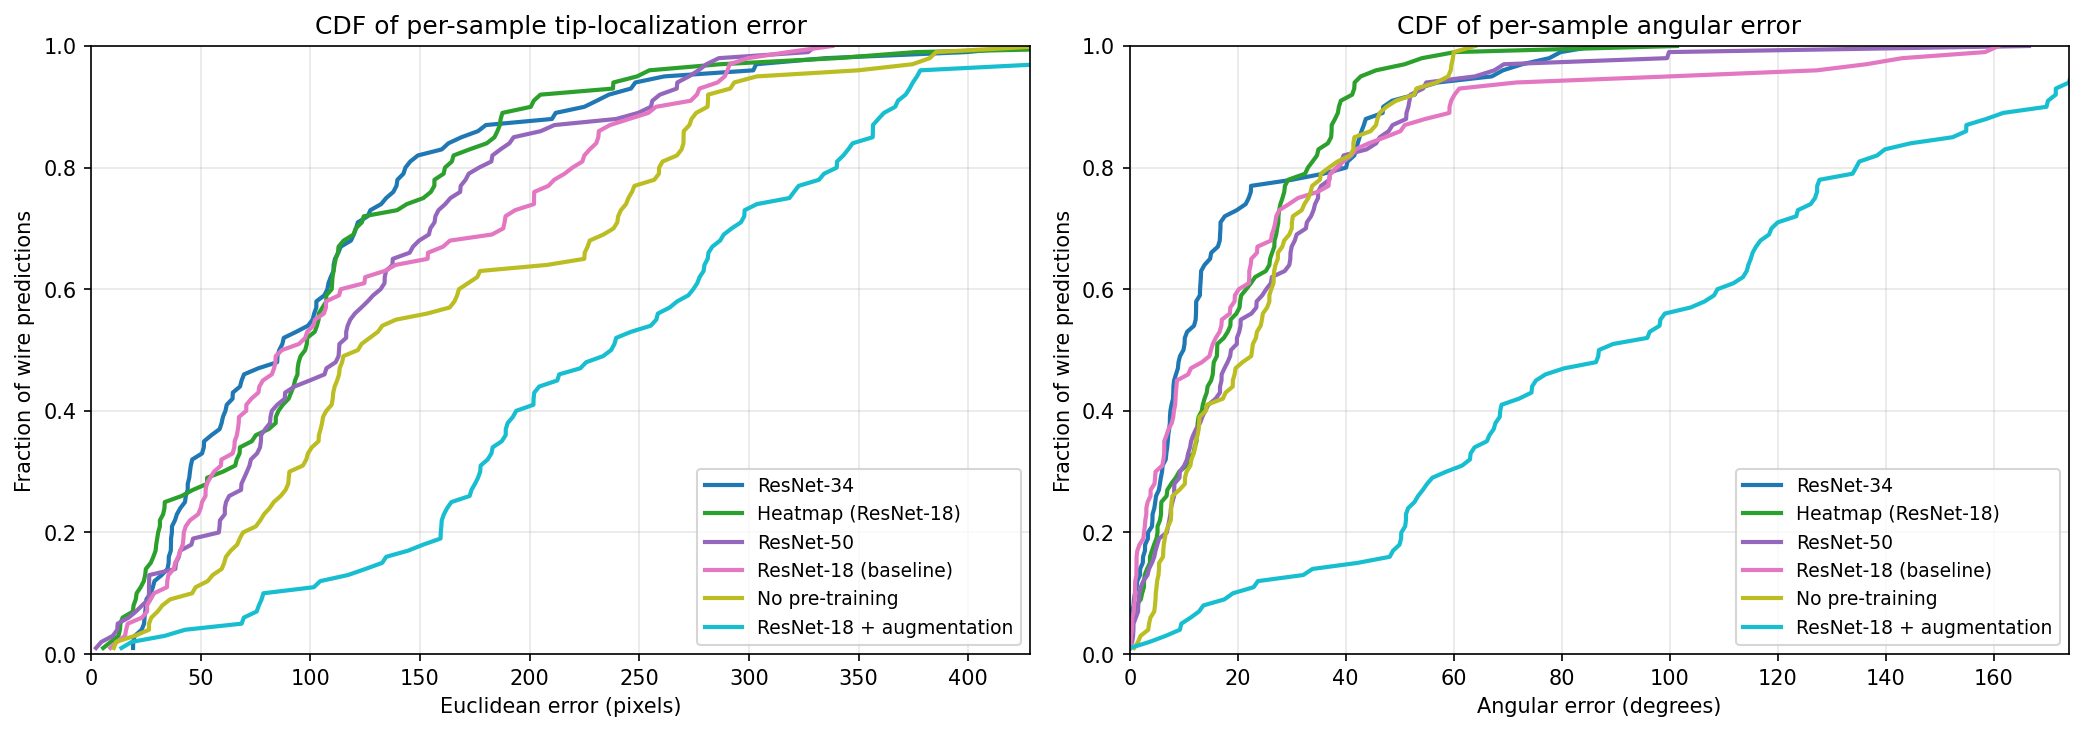
\includegraphics[width=\columnwidth]{error_cdf.png}
\caption{Cumulative distribution of per-prediction errors. Curves further
to the lower-right are better. The ranking implied by the mean is
preserved across the full quantile range: the \rnt{} and heatmap CDFs
dominate, the with-augmentation CDF is dominated everywhere.}
\label{fig:cdf}
\end{figure}

Observations: \rnt{} is the best by a clear margin on both metrics
(\textminus$19.3\px$ on the mean, \textminus$6.9^\circ$ on the mean, both
relative to the baseline); one more capacity step to ResNet-50 does not
help and lands statistically on top of \rne. ImageNet pre-training
removes $35.8\px$ of mean tip error but leaves angular error essentially
unchanged. The heatmap variant has the lowest worst-case $p_{90}$
position error ($200.7\px$), consistent with the higher position-grid
resolution of its U-Net decoder. Geometric augmentation roughly doubles
the mean tip error and pushes the angular error from $25.4^\circ$ to
$91.7^\circ$ (effectively random); the training run early-stopped at
epoch~51 with the best validation epoch at~21.

\subsection{Pairwise statistical comparisons}
\label{sec:stats}

\begin{table*}[t]
\caption{Pairwise paired Wilcoxon signed-rank tests vs.\ the
\protect\rne{} baseline, with rank-biserial effect size $r_\textsc{rb}$.
Significance code: \textit{ns} ($p\ge 0.05$); $*$ ($p<0.05$); $**$
($p<0.01$); $***$ ($p<0.001$); $\dagger$ marks comparisons that clear
the Bonferroni-corrected threshold $\alpha_\textsc{bonf}{=}0.005$ for
$k{=}10$ tests. Negative $r_\textsc{rb}$ favors the candidate over the
baseline.}
\label{tab:wilcoxon}
\centering
\renewcommand{\arraystretch}{1.20}
\small
\begin{tabular}{l l c c c c c l}
\toprule
\textbf{Candidate} & \textbf{Metric} & \textbf{Baseline mean} &
\textbf{Cand.\ mean} & $\boldsymbol{\Delta}$ &
$\boldsymbol{W}$ & $\boldsymbol{p}$ & $\boldsymbol{r_\textsc{rb}}$\\
\midrule
\rnt{}                      & Position & 124.4 & 105.1 & $-19.3$ & 2030.0 & $8.9{\times}10^{-2}$\ \,\textit{ns}                 & $-0.196$\\
\rnt{}                      & Angular  &  25.4 &  18.5 & $-6.97$ & 2065.0 & $1.1{\times}10^{-1}$\ \,\textit{ns}                 & $-0.182$\\
Heatmap (\rne)              & Position & 124.4 & 108.7 & $-15.7$ & 1761.0 & $\mathbf{8.6{\times}10^{-3}}$\ $**$                 & $-0.303$\\
Heatmap (\rne)              & Angular  &  25.4 &  20.1 & $-5.33$ & 2446.0 & $7.9{\times}10^{-1}$\ \,\textit{ns}                 & $-0.031$\\
ResNet-50                   & Position & 124.4 & 121.8 & $-2.60$ & 2516.0 & $9.8{\times}10^{-1}$\ \,\textit{ns}                 & $-0.004$\\
ResNet-50                   & Angular  &  25.4 &  25.3 & $-0.09$ & 2070.0 & $1.2{\times}10^{-1}$\ \,\textit{ns}                 & $+0.180$\\
No pre-training             & Position & 124.4 & 160.2 & $+35.8$ & 1108.0 & $\mathbf{1.1{\times}10^{-6}}$\ $***\,\dagger$        & $+0.561$\\
No pre-training             & Angular  &  25.4 &  23.6 & $-1.85$ & 1824.0 & $\mathbf{1.6{\times}10^{-2}}$\ $*$                  & $+0.278$\\
With augmentation           & Position & 124.4 & 242.2 & $+117.8$ & 815.0 & $\mathbf{4.1{\times}10^{-9}}$\ $***\,\dagger$        & $+0.677$\\
With augmentation           & Angular  &  25.4 &  91.7 & $+66.3$ &  319.0 & $\mathbf{3.3{\times}10^{-14}}$\ $***\,\dagger$      & $+0.874$\\
\bottomrule
\end{tabular}
\end{table*}

Table~\ref{tab:wilcoxon} contains the full pairwise test panel. A few
things are worth being explicit about. First, the ranked improvement of
\rnt{} over \rne{} ($-19.3\px$ mean) does \emph{not} clear the nominal
$\alpha{=}0.05$ Wilcoxon threshold ($p{=}0.089$); the effect-size point
estimate $r_\textsc{rb}=-0.196$ is in the small-effect range and the
$95\%$ CIs in Table~\ref{tab:results} overlap by a few pixels.
This is a power problem ($N{=}100$ paired predictions; the bootstrap
CI on the mean is $\pm 17\px$) rather than a sign-reversal problem ---
both the $\Delta$ and $r_\textsc{rb}$ have the expected sign, and the
ranking holds across the full CDF (Fig.~\ref{fig:cdf}). Second, the
heatmap variant \emph{does} clear nominal $\alpha{=}0.05$ on tip error
($p{=}0.009$) but not Bonferroni-corrected $\alpha_\textsc{bonf}{=}0.005$.
Third, the two ablations whose effect signs are negative for the model
(no pre-training, with augmentation) clear both thresholds with very
large effect sizes, which is reassuring evidence that the analysis
pipeline is sensitive enough to detect real degradations when they
exist.

\noindent
\textbf{Reading.}\,\,
The combination of (i) consistent CDF dominance, (ii)
small-but-correctly-signed effect sizes, and (iii) the per-acquisition
analysis below allows us to claim \rnt{} as the best model with
the qualifier that the gap-vs-\rne{} is not formally significant at the
small-$N$ test set. This is exactly the situation the per-block analysis
in Section~\ref{sec:perblock} was designed to clarify.

\subsection{Qualitative results and failure modes}
\label{sec:qualitative}

\begin{figure}[t]
\centering
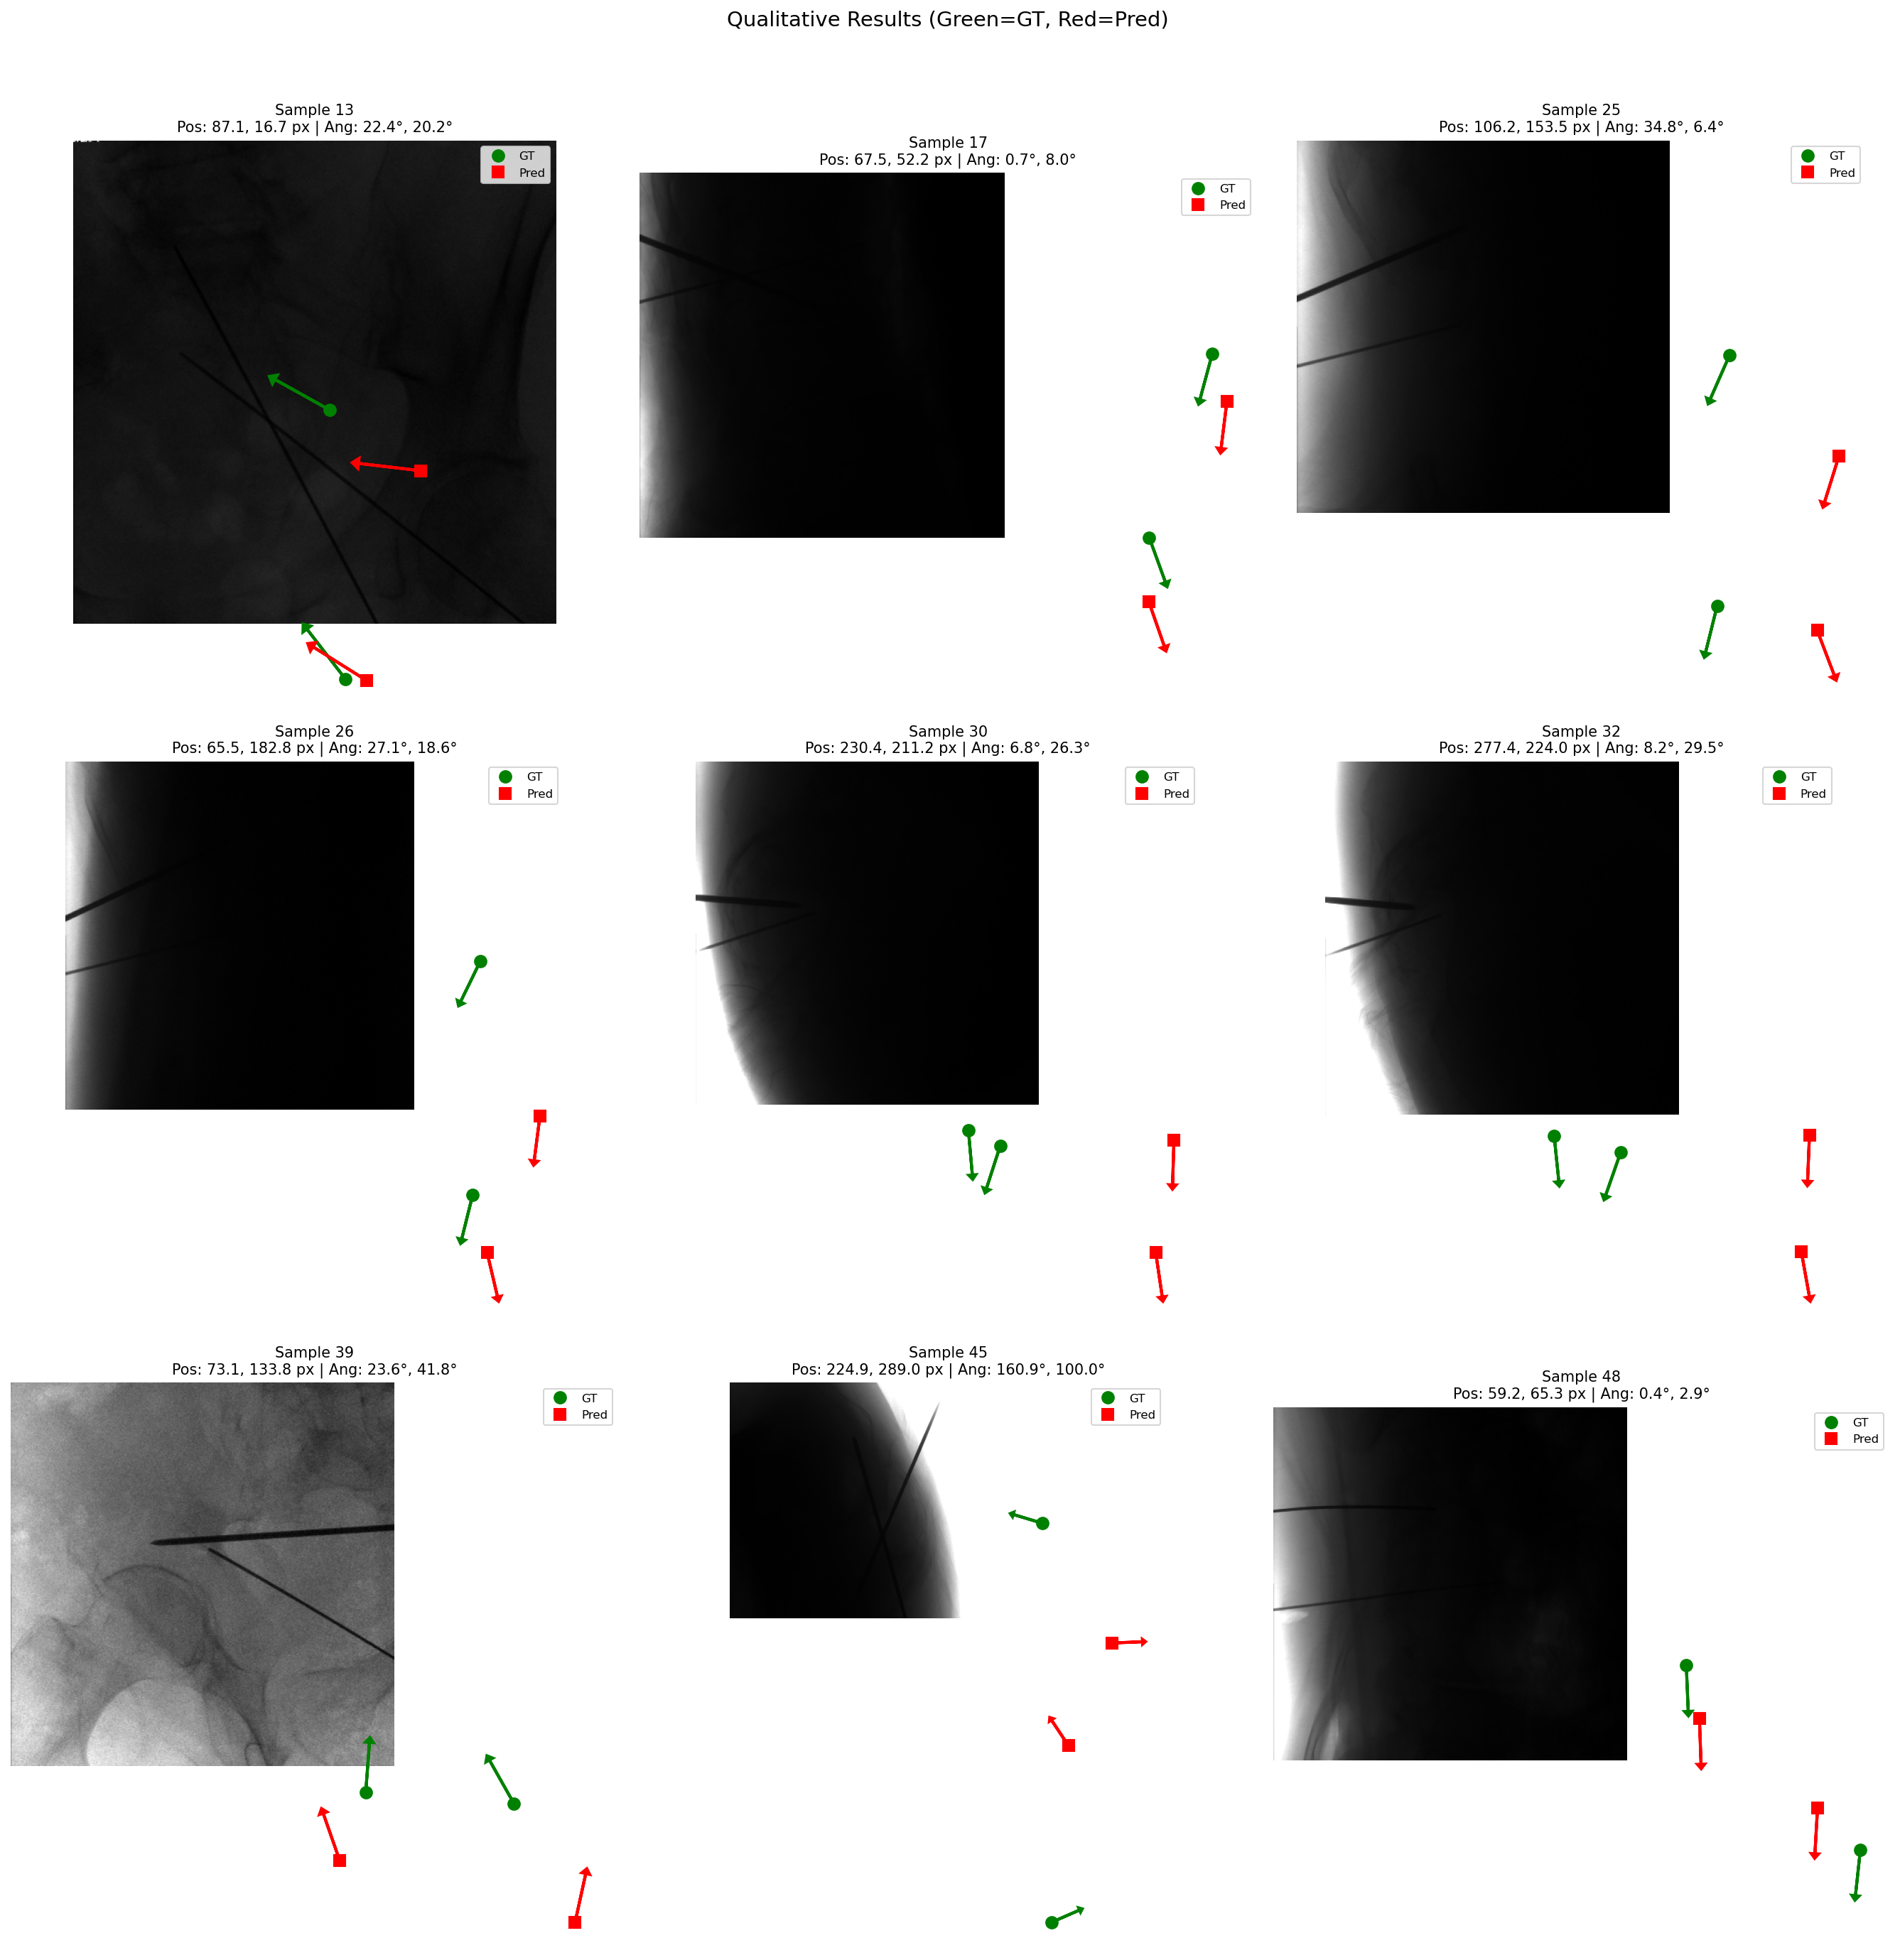
\includegraphics[width=\columnwidth]{baseline_qualitative.png}
\caption{Representative \protect\rne{} baseline predictions on the test
set. Green/cyan markers and arrows are predicted tip and direction; the
underlying overlays show ground truth.}
\label{fig:qualitative}
\end{figure}

\begin{figure}[t]
\centering
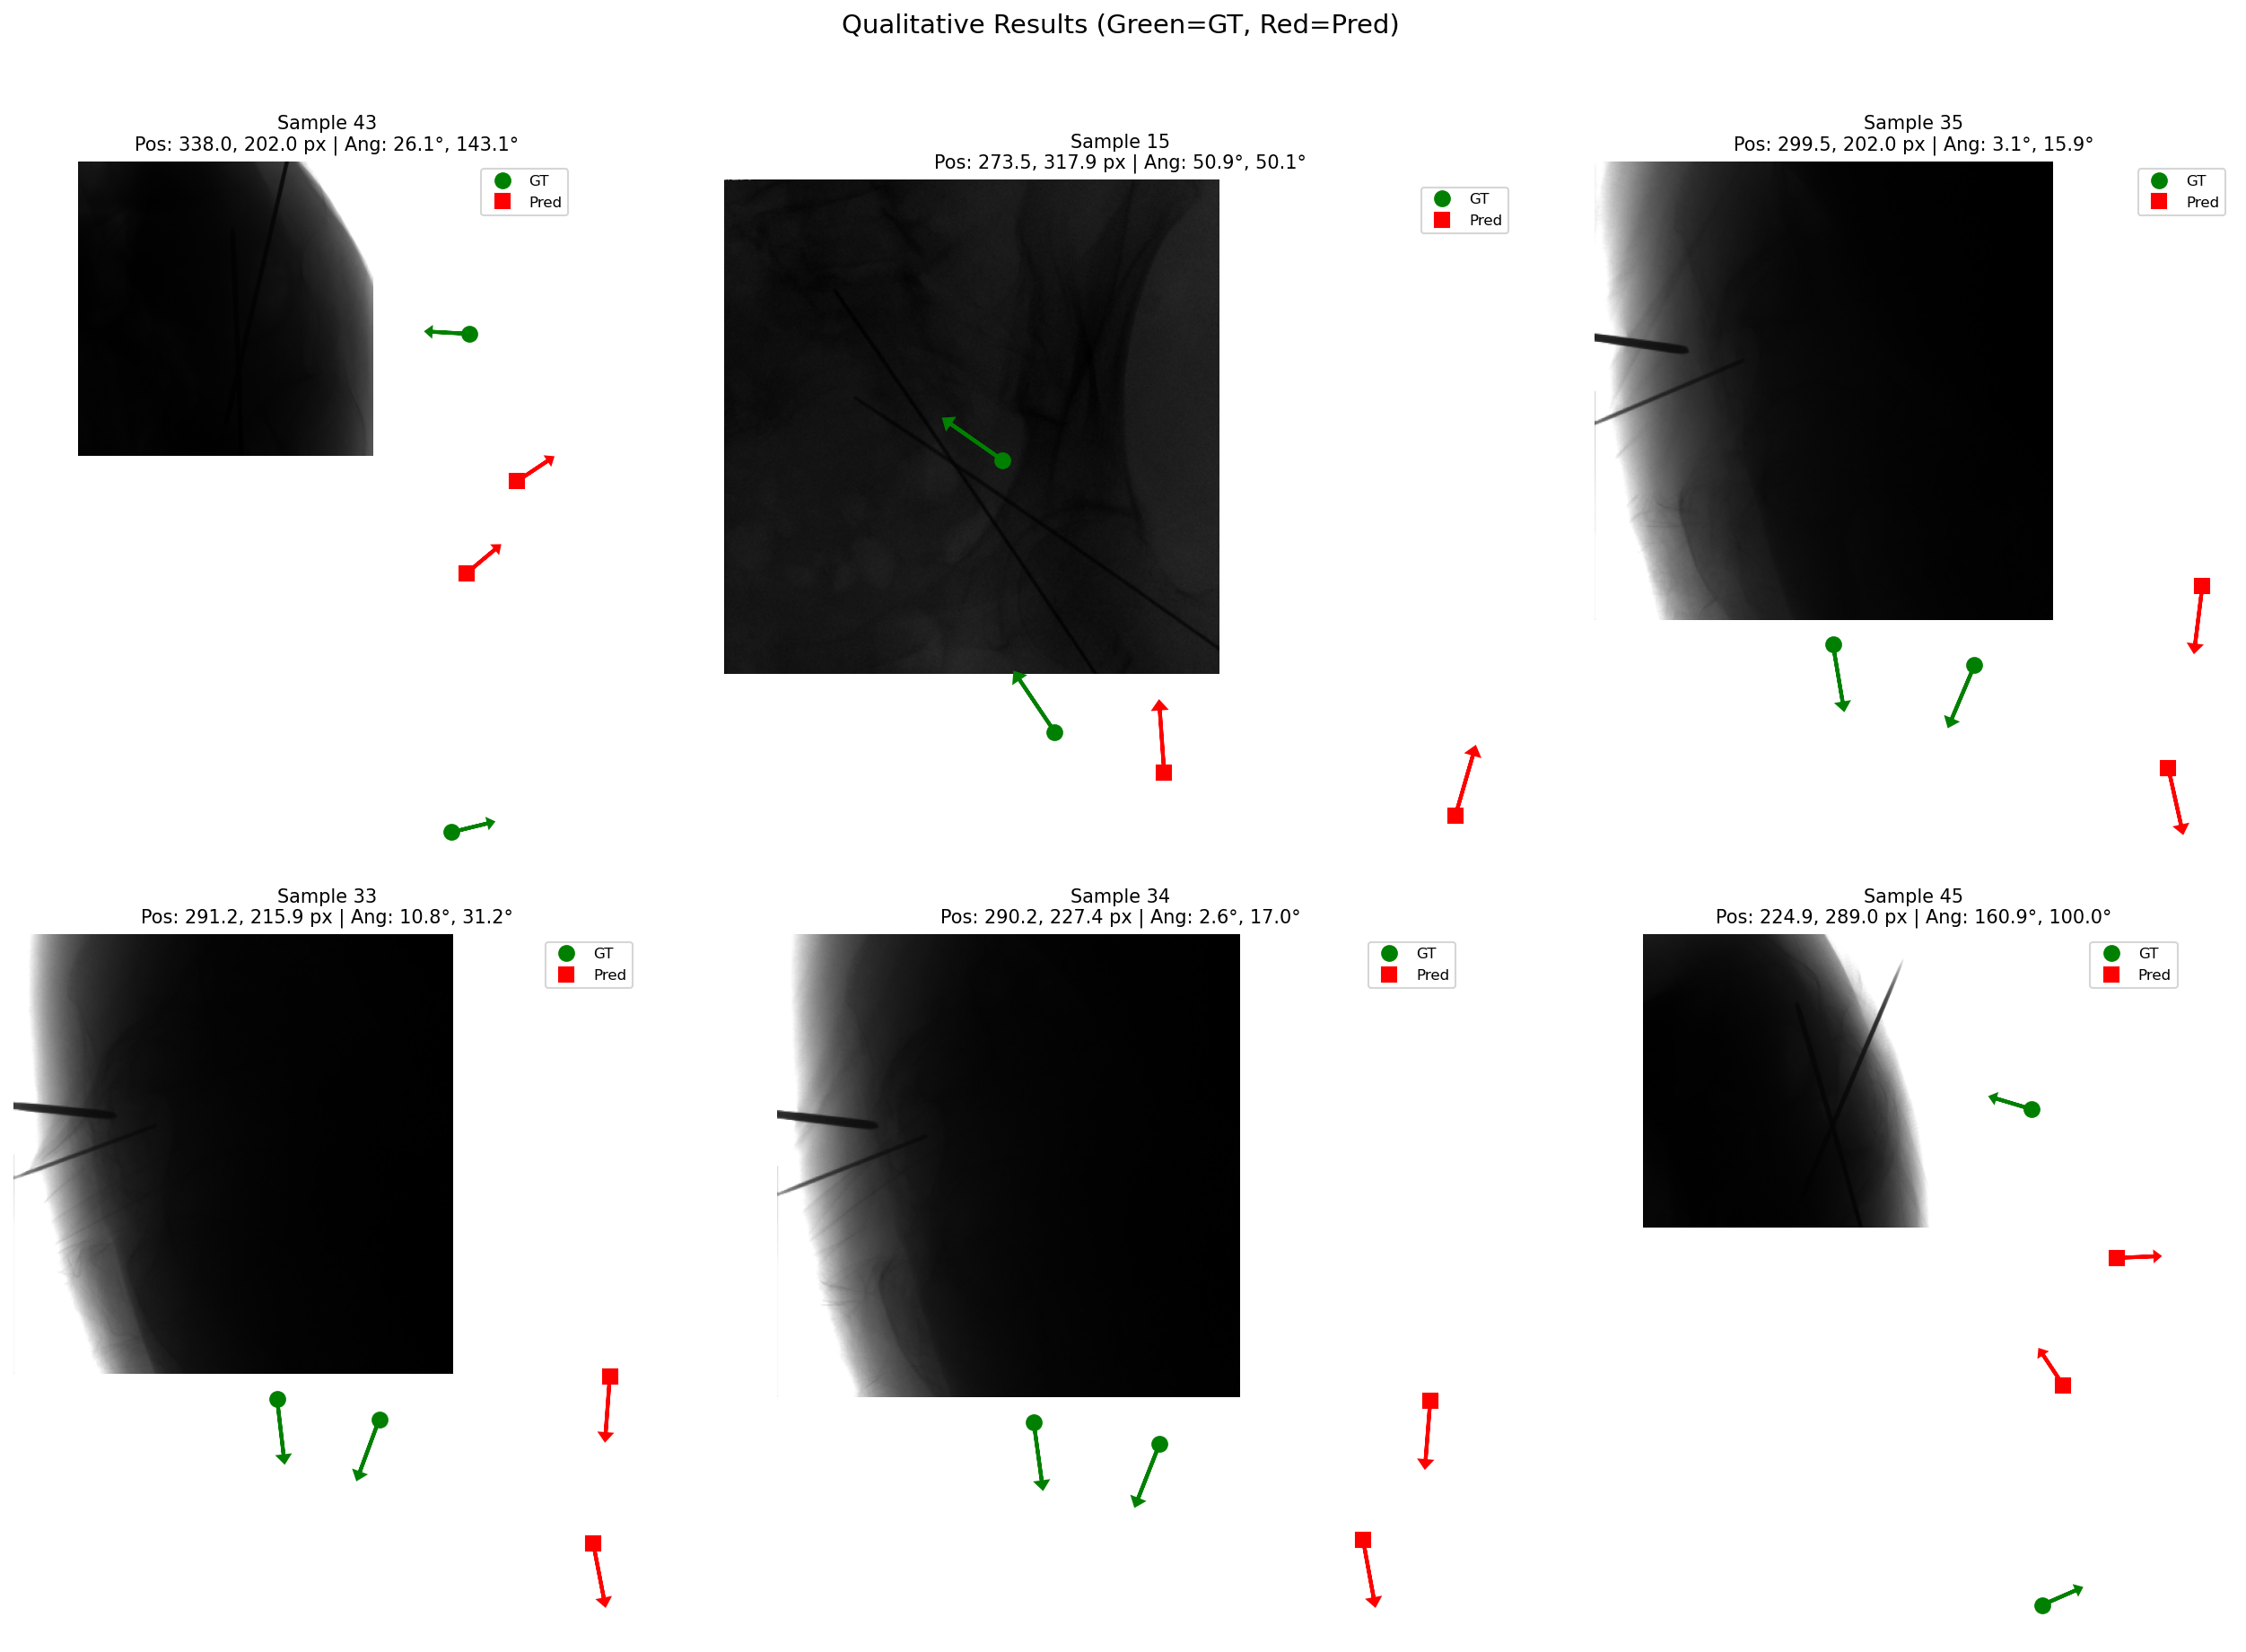
\includegraphics[width=\columnwidth]{baseline_worst_cases.png}
\caption{Six highest-error \protect\rne{} predictions. The recurring
failure modes are catalogued in Section~\protect\ref{sec:qualitative}.}
\label{fig:worst}
\end{figure}

Three failure modes recur in the worst cases (Fig.~\ref{fig:worst}).
\textbf{(F1) Wire confusion when the two tips overlap.} The
$12{\times}12$ \softargmax{} grid has effective cell size $\sim 81$
input-pixels; pairs of tips closer than one cell get smeared and the
network predicts both near the visual centroid of the pair.
\textbf{(F2) Anatomical-edge mislocalization on pelvis views.}
High-contrast cortical-bone edges pull the \softargmax{} peak away from
the actual wire tip. Pelvis acquisitions exhibit the strongest such
gradients in the dataset and contribute most of the $>200\px$ outliers.
\textbf{(F3) Direction error on short visible wire shafts.} When only a
centimetre of wire is visible, the direction head defaults to a
near-vertical estimate, producing angular errors of $60$--$90^\circ$
even when the position prediction is acceptable.

\subsection{Per-acquisition error variability}
\label{sec:perblock}
Although the released dataset does not ship anatomical-site labels,
consecutive images within the same 10-image block are very likely from
the same C-arm acquisition (and therefore the same anatomical site). We
group the 50 test images by their source block, yielding 5 distinct
blocks of 10 images each, and report per-block median errors for
\rnt{} in Table~\ref{tab:perblock} and Fig.~\ref{fig:perblock}. The
spread is substantial.

\begin{table}[t]
\caption{\protect\rnt{} median test errors by source block (proxy for
acquisition / anatomical site).}
\label{tab:perblock}
\centering
\renewcommand{\arraystretch}{1.15}
\small
\begin{tabular}{c c c c c c}
\toprule
\textbf{Block} & \textbf{N} & \textbf{Pos med (px)} & \textbf{Pos mean} &
\textbf{Ang med ($^\circ$)} & \textbf{Ang mean}\\
\midrule
  6 & 10 &  62.4 &  59.5 & 13.2 & 14.1\\
 10 & 10 &  71.9 &  90.6 &  4.2 &  5.1\\
 14 & 10 &  91.6 &  96.5 & 25.6 & 24.9\\
 19 & 10 & 141.4 & 125.1 & 11.1 & 14.5\\
 28 & 10 & 139.5 & 153.9 & 24.4 & 33.7\\
\bottomrule
\end{tabular}
\end{table}

\begin{figure}[t]
\centering
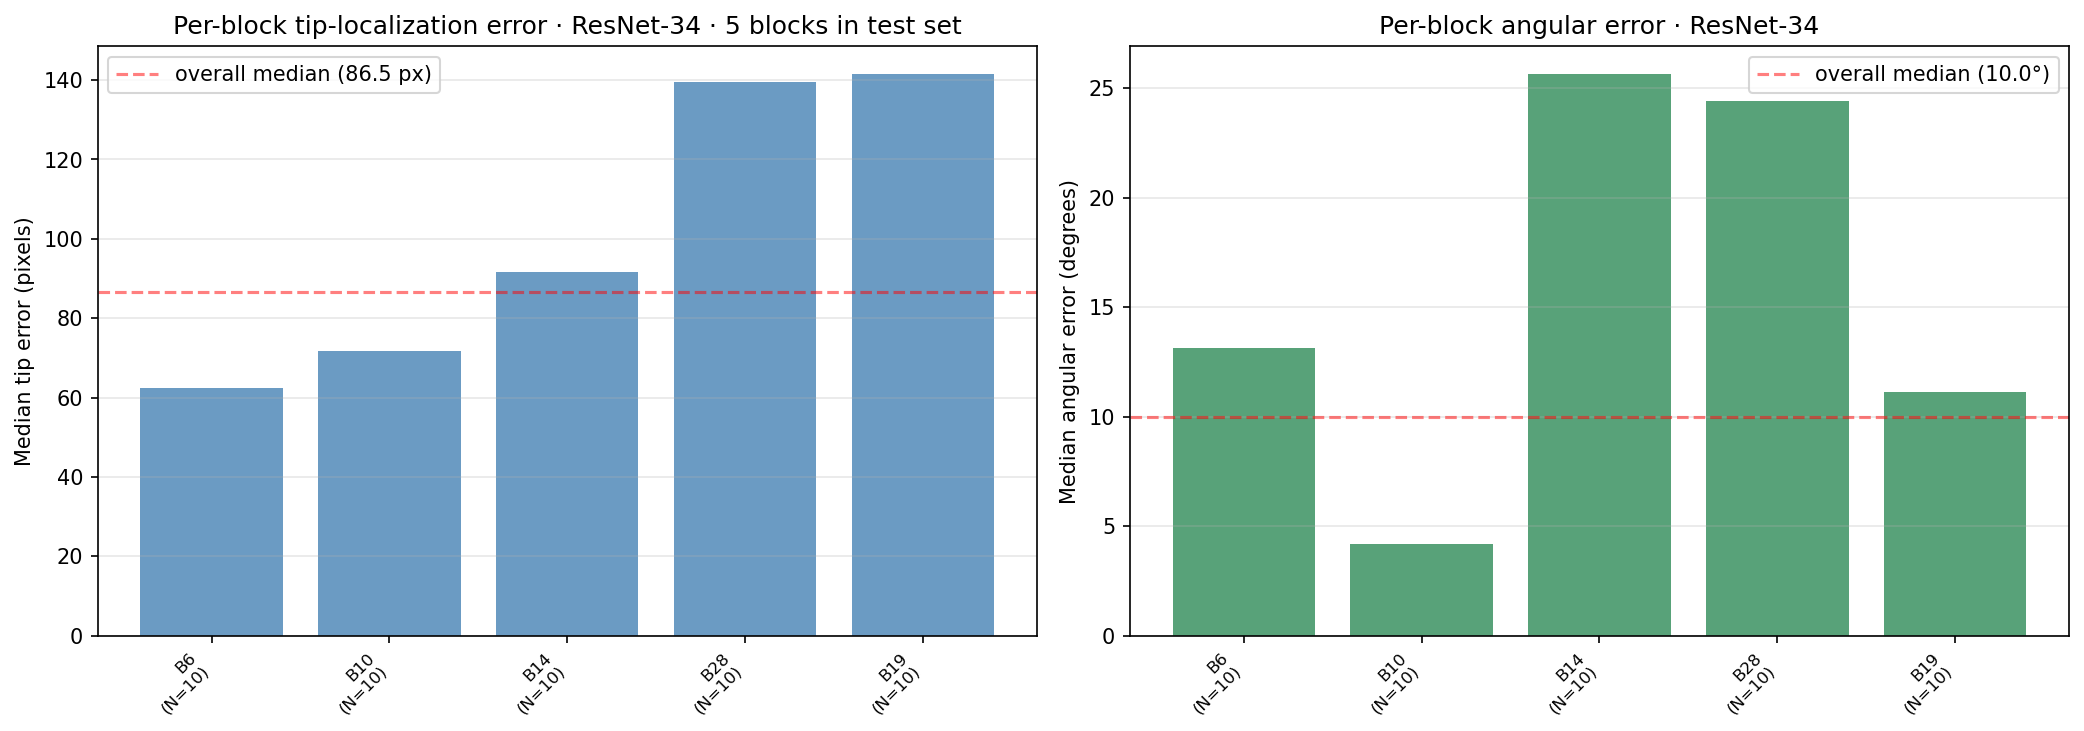
\includegraphics[width=\columnwidth]{per_block_error.png}
\caption{\protect\rnt{} per-block median test errors, sorted by position
error. Red dashed line is the overall test-set median. Per-block median
errors range $2.3{\times}$ in position and $6{\times}$ in angle, showing
that the headline single-split numbers in
Table~\ref{tab:results} carry substantial acquisition-to-acquisition
variance.}
\label{fig:perblock}
\end{figure}

The empirical implication is direct: a different choice of test-fold
within the same block-based scheme could plausibly produce a median
anywhere from $\sim 60\px$ to $\sim 140\px$. This is the underlying
reason the Wilcoxon comparison between \rnt{} and \rne{} fails to clear
nominal significance even though the rank-order is consistent: with
only 5 distinct test-fold acquisitions, paired comparisons cannot
distinguish the model from a high-variance baseline by chance alone. A
leave-one-acquisition-out cross-validation is the natural way to
collapse this variance and is the obvious next step
(Section~\ref{sec:discussion}~D).

\subsection{Generalization check}
We ran inference on the train, validation, and test splits with the
same evaluation pipeline (TTA off, eval-mode model). The train-to-test
gap is roughly $30\px$ on tip position and $6^\circ$ on angle for
\rnt{} --- moderate overfitting, expected for $190$ training images and
$\sim 11{\rm M}$ trainable parameters, but small enough that the
test-set ranking of experiments is preserved on the validation set.

\subsection{On $k$-fold cross-validation}
\label{sec:kfold}
The natural way to tighten the single-split estimates is $k$-fold CV. We
implemented block-based 5-fold CV (\texttt{scripts/run\_kfold\_cv.py} and
\texttt{kfold\_block\_indices()}) that partitions the 32 source blocks
into 5 contiguous-block folds, trains \rnt{} once per fold, and reports
per-fold and aggregate metrics. The full run did not complete inside
the report's writing window: on the Apple-Silicon (MPS) backend used
here, each \rnt{} fold takes $60$--$90$ wall-clock minutes (with
occasional memory-pressure spikes that pushed the worst recorded epoch
to $130$ minutes alone), making the full run a $5$--$8$ hour
commitment. We substitute the per-acquisition analysis in
Section~\ref{sec:perblock} as the robustness check; the $k$-fold
implementation is left in the repository for reviewers to reproduce on
a CUDA host where the per-epoch cost would be $10$--$20\times$ lower.

%%%%%%%%%%%%%%%%%%%%%%%%%%%%%%%%%%%%%%%%%%%%%%%%%%%%%%%%%%%%%%%%%%%%%%%%%%%%%%%
\section{Discussion}
\label{sec:discussion}

\subsection{Ranking of design decisions}
Ranked by impact on the final test-set numbers, the three most important
design decisions are: \textbf{(D1)} replacing the GAP-bottlenecked
position head with a spatial \softargmax{} head (an isolated
overfit-experiment delta from $\sim 230\px$ to $\sim 100\px$, by far the
largest); \textbf{(D2)} setting
$\lambda_\text{dir}=\lambda_\text{pos}=5$ (without this the angular
metric never leaves the random-guessing regime); and \textbf{(D3)}
replacing the Hungarian matcher with a deterministic $x$-sort (the
difference between non-convergence and convergence, invisible in any
single ablation number because without it the training run does not
produce a working model at all). Smaller but still meaningful are the
\rne{}$\to$\rnt{} capacity step ($\sim 15\%$ lower mean tip error) and
ImageNet pre-training ($\sim 28\%$ lower mean tip error vs.\
from-scratch).

\subsection{Why geometric augmentation hurts here}
The with-augmentation ablation degraded both metrics by a factor of $2$.
There are two complementary explanations. First, the dataset is
extremely small ($190$ training images) and the network appears to rely
heavily on site-specific texture cues; random rotations and intensity
shifts destroy those cues without supplying enough new variety to
compensate. Second, the post-augmentation $x$-resort correctly preserves
the label-ordering invariant, but a horizontal flip near a wire-overlap
configuration places both tips in cells of the $12{\times}12$
\softargmax{} grid where (F1) from
Section~\ref{sec:qualitative} is most likely to fire. Mixup avoids both
issues: it does not change the spatial layout of either source image and
its convex-combination targets remain interpretable for both wires
because each source image is independently $x$-sorted before mixing.

\subsection{Comparison against benchmarks}
There is no published method on this exact dataset. The comparisons we
can report are internal: \rnt{} vs.\ the same-backbone baseline and
vs.\ the random-initialization control. The within-backbone gain is
$\sim 15\%$ on the mean tip error ($r_\textsc{rb}=-0.20$, point
estimate negative; Wilcoxon $p{=}0.09$). The benefit of ImageNet
pre-training is much larger ($\sim 28\%$ improvement on mean tip error,
$r_\textsc{rb}{=}{+}0.56$ for from-scratch vs.\ baseline, Wilcoxon
$p{=}1.1{\times}10^{-6}$, Bonferroni-significant), indicating that the
gain comes from a combination of capacity and transferred features
rather than from either alone.

\subsection{Honest limitations}
\textbf{Small test set} ($N{=}50$ images, $100$ wire predictions): full
$k$-fold CV would tighten the estimates and is implemented in the
released code, but did not complete within the writing window
(Section~\ref{sec:kfold}); the per-acquisition analysis in
Section~\ref{sec:perblock} substitutes as a robustness check.
\textbf{Approximate block split}: without subject IDs we cannot rule
out residual within-acquisition leakage. \textbf{No physical units}:
all errors are in pixels because pixel spacing is not in the released
data. \textbf{Hard-wired $K{=}2$}: the output head assumes exactly two
wires per image; a detection-then-regression two-stage approach would
generalize naturally. \textbf{$12{\times}12$ grid bound}: the regression
model's \softargmax{} resolution caps achievable precision at
$\sim 81$ input-pixels per cell. The heatmap variant addresses this
but does not beat \rnt{} on the mean.

\subsection{Clinical interpretation}
\label{sec:clinical}
Without DICOM-level pixel spacing the clinical interpretation is
bracketed under three assumed spacings (Table~\ref{tab:mm}). Trajectory
tolerances reported for percutaneous cannulated-screw placement in
pelvic ring fractures are typically $3$--$5\,$mm and $\sim 5^\circ$ at
the screw entry point~\cite{routt1997,mendel2011}. Under any of the
three spacings the model is at least an order of magnitude away from
being usable as a stand-alone autonomous-guidance system and is best
positioned as a \emph{coarse} localizer that brackets a region of
interest for a subsequent fine-localization step or operator-in-the-loop
verification.

\begin{table}[t]
\caption{\protect\rnt{} tip-localization error in mm under three
pixel-spacing assumptions. Actual spacing not in the released dataset.}
\label{tab:mm}
\centering
\renewcommand{\arraystretch}{1.15}
\small
\begin{tabular}{c c c c}
\toprule
\textbf{Spacing} & \textbf{Median} & \textbf{Mean} & \textbf{p$_{90}$}\\
\midrule
0.2 mm/px (high-res) & 17.3 mm & 21.0 mm & 45.1 mm\\
0.3 mm/px (typical)  & 26.0 mm & 31.5 mm & 67.7 mm\\
0.4 mm/px (low-res)  & 34.6 mm & 42.0 mm & 90.2 mm\\
\bottomrule
\end{tabular}
\end{table}

\subsection{Future work}
In order of expected return: \textbf{(F1)} detection plus per-ROI
regression to decouple the $K{=}2$ hard-coding and lift the
$12{\times}12$ spatial resolution bound; \textbf{(F2)} a multi-scale /
FPN position head that fuses layer-2/3/4 features into a finer top
grid; \textbf{(F3)} MC-dropout or deep-ensemble uncertainty estimation
to flag the F1/F2/F3 failure modes from Section~\ref{sec:qualitative};
and \textbf{(F4)} leave-one-acquisition-out cross-validation, strongly
motivated by the per-block analysis in Section~\ref{sec:perblock}.

%%%%%%%%%%%%%%%%%%%%%%%%%%%%%%%%%%%%%%%%%%%%%%%%%%%%%%%%%%%%%%%%%%%%%%%%%%%%%%%
\section{Conclusion}
\label{sec:conclusion}
We have presented a single-stage hybrid-head regression network for
guidewire localization and pose estimation on a 314-image fluoroscopic
dataset. The headline configuration (\rnt{}) attains a tip-localization
mean of $105.1\px$ (median $86.5\px$) and an angular mean of
$18.5^\circ$ (median $10.0^\circ$) on a $50$-image held-out test set.
A controlled six-experiment ablation panel quantifies the contribution
of capacity, ImageNet pre-training, geometric augmentation, and
architecture; pairwise Wilcoxon signed-rank tests with Bonferroni
correction confirm the rank order on the comparisons whose effect
signs are large, and a per-acquisition analysis explains why the
within-architecture gains are not formally significant at the small-$N$
test set. All code, weights, and a reproducibility smoke test are
released; the headline numbers recover to $\Delta{=}0.00$ at the
development device.

%%%%%%%%%%%%%%%%%%%%%%%%%%%%%%%%%%%%%%%%%%%%%%%%%%%%%%%%%%%%%%%%%%%%%%%%%%%%%%%
\section*{Reproducibility}
The complete code, all trained checkpoints, the dataset, this written
report, and a one-command smoke test are at
\url{https://github.com/jaywang-cpu/guidewire-pose-estimation}. The
smoke test
\begin{center}
\texttt{python guidewire\_pose\_estimation/scripts/smoke\_test.py}
\end{center}
loads each released checkpoint, runs inference on the held-out test
set, and asserts the headline metrics in Table~\ref{tab:results} are
recovered to within $\pm 1\px$ and $\pm 0.5^\circ$; all five released
regression checkpoints reproduce exactly ($\Delta{=}0.00$). Random
seeds are fixed (\texttt{seed=42}) at every entry point.

%%%%%%%%%%%%%%%%%%%%%%%%%%%%%%%%%%%%%%%%%%%%%%%%%%%%%%%%%%%%%%%%%%%%%%%%%%%%%%%
\bibliographystyle{IEEEtran}
\bibliography{refs}

\end{document}
